\chapter{Codierungstheorie}

\section{Grundbegriffe und einfache Beispiele}

\subsection{Codierung} (Kanalcodierung)\\
Sicherung von Daten/Nachrichten gegen zuf\"allig auftretenden Fehler bei Speicherung/\"Ubertragung.\\
\begin{figure}[h]
	\centering
	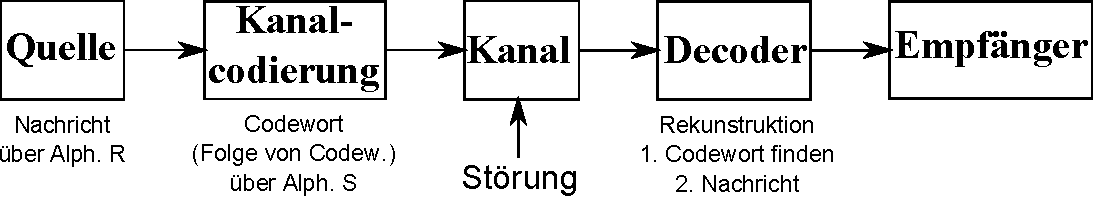
\includegraphics[totalheight=0.1\textheight]{./img/codierung_schaubild.pdf}
	\caption{Schaubild der Codierung}
	\label{img:Schaubild Codierung}
\end{figure}

\subsection{Ziele}
\begin{itemize}
	\item M\"oglichst viele Fehler erkennen und gegebenenfalls korrigieren. %ABKUERZUNG
	\item Aufwand f\"ur Codierung und Decodierung m\"oglichst gering.
\end{itemize}

\section{Grundprinzip} Hinzuf\"ugen von Redundanz\\
\\
Es gibt zwei Typen um Redundanz zu erzeugen.
\subsection{FEC-Verfahren (Forward Error Correction)}
Aufgetretene Fehler sollen erkannt \underline{und} korrigiert werden.\\
Vorteil: keine Verz\"ogerung der \"Ubertragung aber ggf. gro\ss e Redundanz notwendig.

\subsection{ARQ-Verfahren (Automatic Repeat Request)}
Aufgetretene Fehler sollen erkannt werden, werden nicht korrigiert. Stattdessen  wiederholt die \"Ubertragung beim Sender anfordern.\\
\\
Vorteil: geringe Redundanz, aber Verz\"ogerung.\\
\\
\subsubsection{Beispiele}
\begin{enumerate}
\item Parity-Check-Codes\\
z.B. Nachrichten: 00, 01, 10, 11\\
\\
Codierung: 00 $\rightarrow$ 000\\
01 $\rightarrow$ 011\\
10 $\rightarrow$ 101\\
11 $\rightarrow$ 110\\
(gerade Anzahl von Einsen in den Codew\"ortern)\\
\\
1 Fehler wird erkannt, nicht korrigiert.\\
2 Fehler werden nicht erkannt.

\item Wiederholungscode\\
Nachrichten wie in 1.\\
\\
Codierung: 00 $\rightarrow$ 000000
01 $\rightarrow$ 010101\\
10 $\rightarrow$ 101010\\
11 $\rightarrow$ 111111\\
(3-Fache Wiederholung)\\
\\
1 Fehler wird erkannt und korrigiert.\\
\underline{01}01\underline{01} $\rightarrow$ 010101 $\rightarrow$ 01
\item Nachrichten wie in 1.
Codierung: 00 $\rightarrow$ 00000\\
01 $\rightarrow$ 01101\\
10 $\rightarrow$ 10110\\
11 $\rightarrow$ 11011\\
\\
Je zwei Codew\"orter unterscheiden sich an mindestens 3 Positionen.\\
Angenommen 1 Fehler tritt bei \"Ubertragung auf. Dann gibt es genau ein Codewort, dass sich vom empfangenen Wort an genau einer Stelle unterscheidet; in das wird decodiert.\\
\\
Muss immer Ungerade unterschiede in Codew\"ortern sein. Bei 5 diffs sind 2 Fehler korrigierbar.
\item (ehmaliger) ISBN-Code
International Standard Book Number\\
\\
10-Stelliger Code\\
Erste 9 Ziffern haben inhaltliche Bedingung ($\entspricht$ Nachricht)\\
10. Ziffer: Pr\"ufziffer\\
\\
Beispiel: 3-540-26121-? (Land - Verlag - Buchnummer - Pr\"ufziffer)\\
\\
Uncodierte W\"orter sind gebildet \"uber $R=\{0, \ldots, 9\}$\\
Codierte W\"orter sind gebildet \"uber $S=\{0, \ldots, 9, X\}$\\
\\
ISBN-Wort $C_{10}C_9\ldots C_2C_1$\\
$C_{10}\ldots C_2$ inhaltliche Bedingung, $C_1$ wird so gew\"ahlt, dass
\[
	\sum^{10}_{k=1} k \cdot C_k \equiv 0 (\md 11)
\]

$10\cdot C_{10}+\ldots + 2\cdot C_2 + C_1 \equiv 0(\md 11)$ falls $C_1 = 10$ so setzte $C_1 = X$\\
$C_1$ vom Beispiel ausrechnen.\\
\\
$ 10\cdot 3+9\cdot 5+8\cdot 4+7\cdot 0+6\cdot 2+5\cdot 6+4\cdot 1+3\cdot 2+2\cdot 1+C_1 = 0 (\md 11)$\\
$ 161 + C_1 = 0 (\md 11) \Rightarrow C_1 = 4$\\
\\
\"Andern einer Ziffer wird erkannt:\\
$C_{10} C_9\ldots C_2 C_1 \rightarrow\ C_i$ wird $X_i \neq C_i$ ersetzt\\
$C_{10} \ldots C_{i+1} X_i C_{i-1} \ldots C_1$
\[
	\sum^{10}_{k=1, k \neq i} k \cdot C_k + i \cdot x_i = 
	\underbrace{\sum^{10}_{k=1, k \neq i} k \cdot C_k}_{\equiv 0 (\md 11)}
	\overbrace{
			\underset{\underset{\nequiv 0 (\md 11)}{\uparrow}}{i} 
			\cdot (\underbrace{x_i-c_i}_{\nequiv 0 (\md 11)}) 
	}^{\nequiv 0 (\md 11)}
	\nequiv 0(\md 11)	
\]
Fehler wird erkannt, Korrektur nicht m\"oglich.\\
\\
$3-540-26121-4 \equiv 0(\md 11)$\\ \\
$\left.
\begin{matrix}
	3-540-26121-\mathbf{6} \\
	3-540-2612\mathbf{2}-4
\end{matrix}
\right\} \text{Pr\"ufsumme 2.}
$\\

Vertauschung von Zwei Ziffern wird erkannt.\\
$C_i$ und $C_j$ vertauscht.\\
O.B.d.A $C_i \neq C_j$\\
$C_{10} \ldots \underset{\stackrel{\uparrow}{i}}{C_j} \ldots \underset{\stackrel{\uparrow}{j}}{C_i} \ldots C_1$\\
\[
	\sum^{10}_{k=1, k\neq i,j} k \cdot C_k + i \cdot 	C_j + j \cdot C_i
	= \sum^{10}_{k=1} k \cdot C_k + i(C_j-C_i)+j(C_i-C_j)
\]
\[
	= 
	\underbrace{\sum^{10}_{k=1} k \cdot C_k}_{\equiv 0 (\md 11)}
	 + 
	 \underbrace{(C_j-C_i)}_{\nequiv 0 (\md 11)}
	 \underbrace{(i-j)}_{\nequiv 0 (\md 11)}
	 \nequiv 0 (\md 11)
\]
Vertauschung wird durch gewichtete Quersummen erkannt.


\item EAN-13-Code\\
\\
European Article Number\\
13-Stelliger Code, erste 12 Ziffer sind inhaltlich festgelegt.\\
13. Ziffer ist Pr\"ufziffer.\\
$R=S=\{ 0, \ldots, 9\}$ \\
$C_1 \ldots C_{12}C_{13}$\\
\\
$C_1 \ldots C_{12}$ inhaltliche Angabe (in der Regel):\\
$C_1C_2$ Herstellerland (40-43 Deutschland)\\
$C_6 \ldots C_7$ Hersteller
$C_8 \ldots C_12$ interne Produktions Nummer\\
\\
$C_{13}$ so gew\"ahlt, dass\\
\[
	C_1 + 3\cdot C_2 + C_3 + 3\cdot C_4 + \ldots + 3\cdot C_{12} + C_{13} \equiv 0 (\md 10)
\]
$x \rightarrow 3x$ Permutation auf $\Z_{10} (\md 10)$, da ggT(3,10)=1\\ %FORMATTING vom ggT?
1 Fehler wird erkannt. Vertauschung in der Regel nicht erkannt. \\
\\
\"Ubersetzung in Barcode: \\
$C_1 C_2 \ldots C_7 C_8 \ldots C_{13}$\\
\\
Jede der Ziffern $C_2, \ldots, C_{13}$ wird durch einen 0-1-String der L\"ange 7 bin\"ar codiert. \\
$0 \entspricht$ wei�er Balken, $1 \entspricht$ schwarzer Balken. \\
Codierung sorgt daf\"ur, dass nie mehr als 4 wei�e oder schwarze Balken nebeneinander stehen. \\

\newpage

\begin{figure}[h]
	\centering
	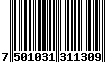
\includegraphics[totalheight=0.1\textheight]{./img/ean13.png}
	\caption{EAN-13 Barcode}
	\label{img:EAN-13 Barcode}
\end{figure}

Schmalen Balken in Mitte und am Rand, sind nur Abtrennzeichen, die nichts mit EAN zu tun haben und nur beim einscannen helfen.\\
5 zu $0110001_2$ \\
\\
$C_2,\ldots, C_7$ werden nach Code A oder Code B codiert. $C_1$ bestimmt welcher dieser beiden Codes verwendet wird. \\
$C_8,\ldots, C_{13}$ werden nach Code C codiert.\\
$C_1$ ergibt sich aus der Art der Codierung von $C_2,\ldots,C_7$

%Table shit here
\begin{center}
	\begin{tabular}{| c | c | c | c | p{2cm} |}
	\hline
	 &\multicolumn{2}{|c|}{\textbf{Ziffern $\mathbf{C_2 - C_7}$}} & \textbf{Ziffern $\mathbf{C_8 - C_{13}}$} & \textbf{bestimmt durch} $\mathbf{C_1}$ \\
	\hline
	\textbf{Zeichen} & \textbf{Code A} & \textbf{Code B} & \textbf{Code C} & \textbf{Code D}\\
	\hline
	\textbf{0} &	0001101 &	0100111 &	1110010 &	AAAAAA\\
	\textbf{1} &	0011001 &	0110011 &	1100110 &	AABABB\\
	\textbf{2} &	0010011 &	0011011 &	1101100 &	AABBAB\\
	\textbf{3} &	0111101 &	0100001 &	1000010 &	AABBBA\\
	\textbf{4} &	0100011 &	0011101 &	1011100 &	ABAABB\\
	\textbf{5} &	0110001 &	0111001 &	1001110 &	ABBAAB\\
	\textbf{6} &	0101111 &	0000101 &	1010000 &	ABBBAA\\
	\textbf{7} &	0111011 &	0010001 &	1000100 & 	ABABAB\\
	\textbf{8} &	0110111 &	0001001 &	1001000 &	ABABBA\\
	\textbf{9} &	0001011 &	0010111 &	1110100 &	ABBABA\\
	\hline
	\end{tabular}
\end{center}







Codew\"orter von Code A,B oder C kommen nur einmal vor. Daher treten nie mehr als 4 gleiche Balken nebeneinander auf. \\
\end{enumerate}




